\capitulo{1}{Introducción}

SpotMyFM es una plataforma diseñada para gestionar la biblioteca y playlists personales de un usuario de Spotify.

Este proyecto busca estudiar el diseño de Spotify y sus distintos sistemas, como sistemas de recomendación o generación de playlists automáticas. Para llevar a cabo este objetivo se ha decidido implementar en un servicio a parte una expansión de la funcionalidad de Spotify que complemente a los servicios ya existentes, como consultar estadísticas, canciones favoritas o generar playlists específicas a partir de filtros y/o recomendaciones.

La plataforma web incluye 7 servicios diferenciados:
\begin{enumerate}
    \item \textbf{Gestión de Favoritos:} Es la página principal, muestra las canciones y artistas más escuchados en varios intervalos.
    \item \textbf{Gestión de Biblioteca:} Permite explorar todas las características de la biblioteca personal del usuario\footnote{Las canciones marcadas como "Me Gusta"}
    \item \textbf{Gestión de Álbumes:} Permite gestionar y etiquetar los álbumes favoritos del usuario. El sistema de etiquetar álbumes se asemeja a la creación de listas de álbumes. 
    \item \textbf{Gestión de Playlists:} Permite explorar las playlists creadas o marcadas como me gusta por el usuario. Se pueden detallar cada una de las playlists.
    \item \textbf{Análisis de Canción:} Permite subir y analizar una canción cualquiera. El analizador devuelve los géneros, subgéneros y estados de ánimo de la canción, así como 5 canciones similares. 
    \item \textbf{Búsqueda:} Permite buscar a cualquier artista, canción, álbum o playlist y disfrutar de las características que ofrece la plataforma. 
    \item \textbf{Reproductor:} Permite reproducir álbumes o canciones específicas, así como añadir a la cola, saltar o retroceder una canción.
\end{enumerate}


Para implementar todas estas características se ha usado la API pública de LastFM, y se ha desarrollado una arquitectura de contenedores escalables interconectados \ref{fig:arquitectura_contenedores}.

Ludwig es un servicio que permite, a partir del un fragmento de una canción, obtener canciones similares en Spotify, géneros, subgéneros y los estado de ánimo de una canción. Este servicio utiliza redes neuronales convolucionales (CNN) para clasificar las canciones a partir de su representación mediante sus coeficientes cepstrales en la frecuencia de mel.

NextJS actúa como intermediario entre el cliente, Ludwig y la base de datos. Se encarga de la generación de las páginas web, la autenticación de usuario, comunicación con Ludwig y la gestión de las transacciones de la base de datos. 
\begin{figure}
    \centering
    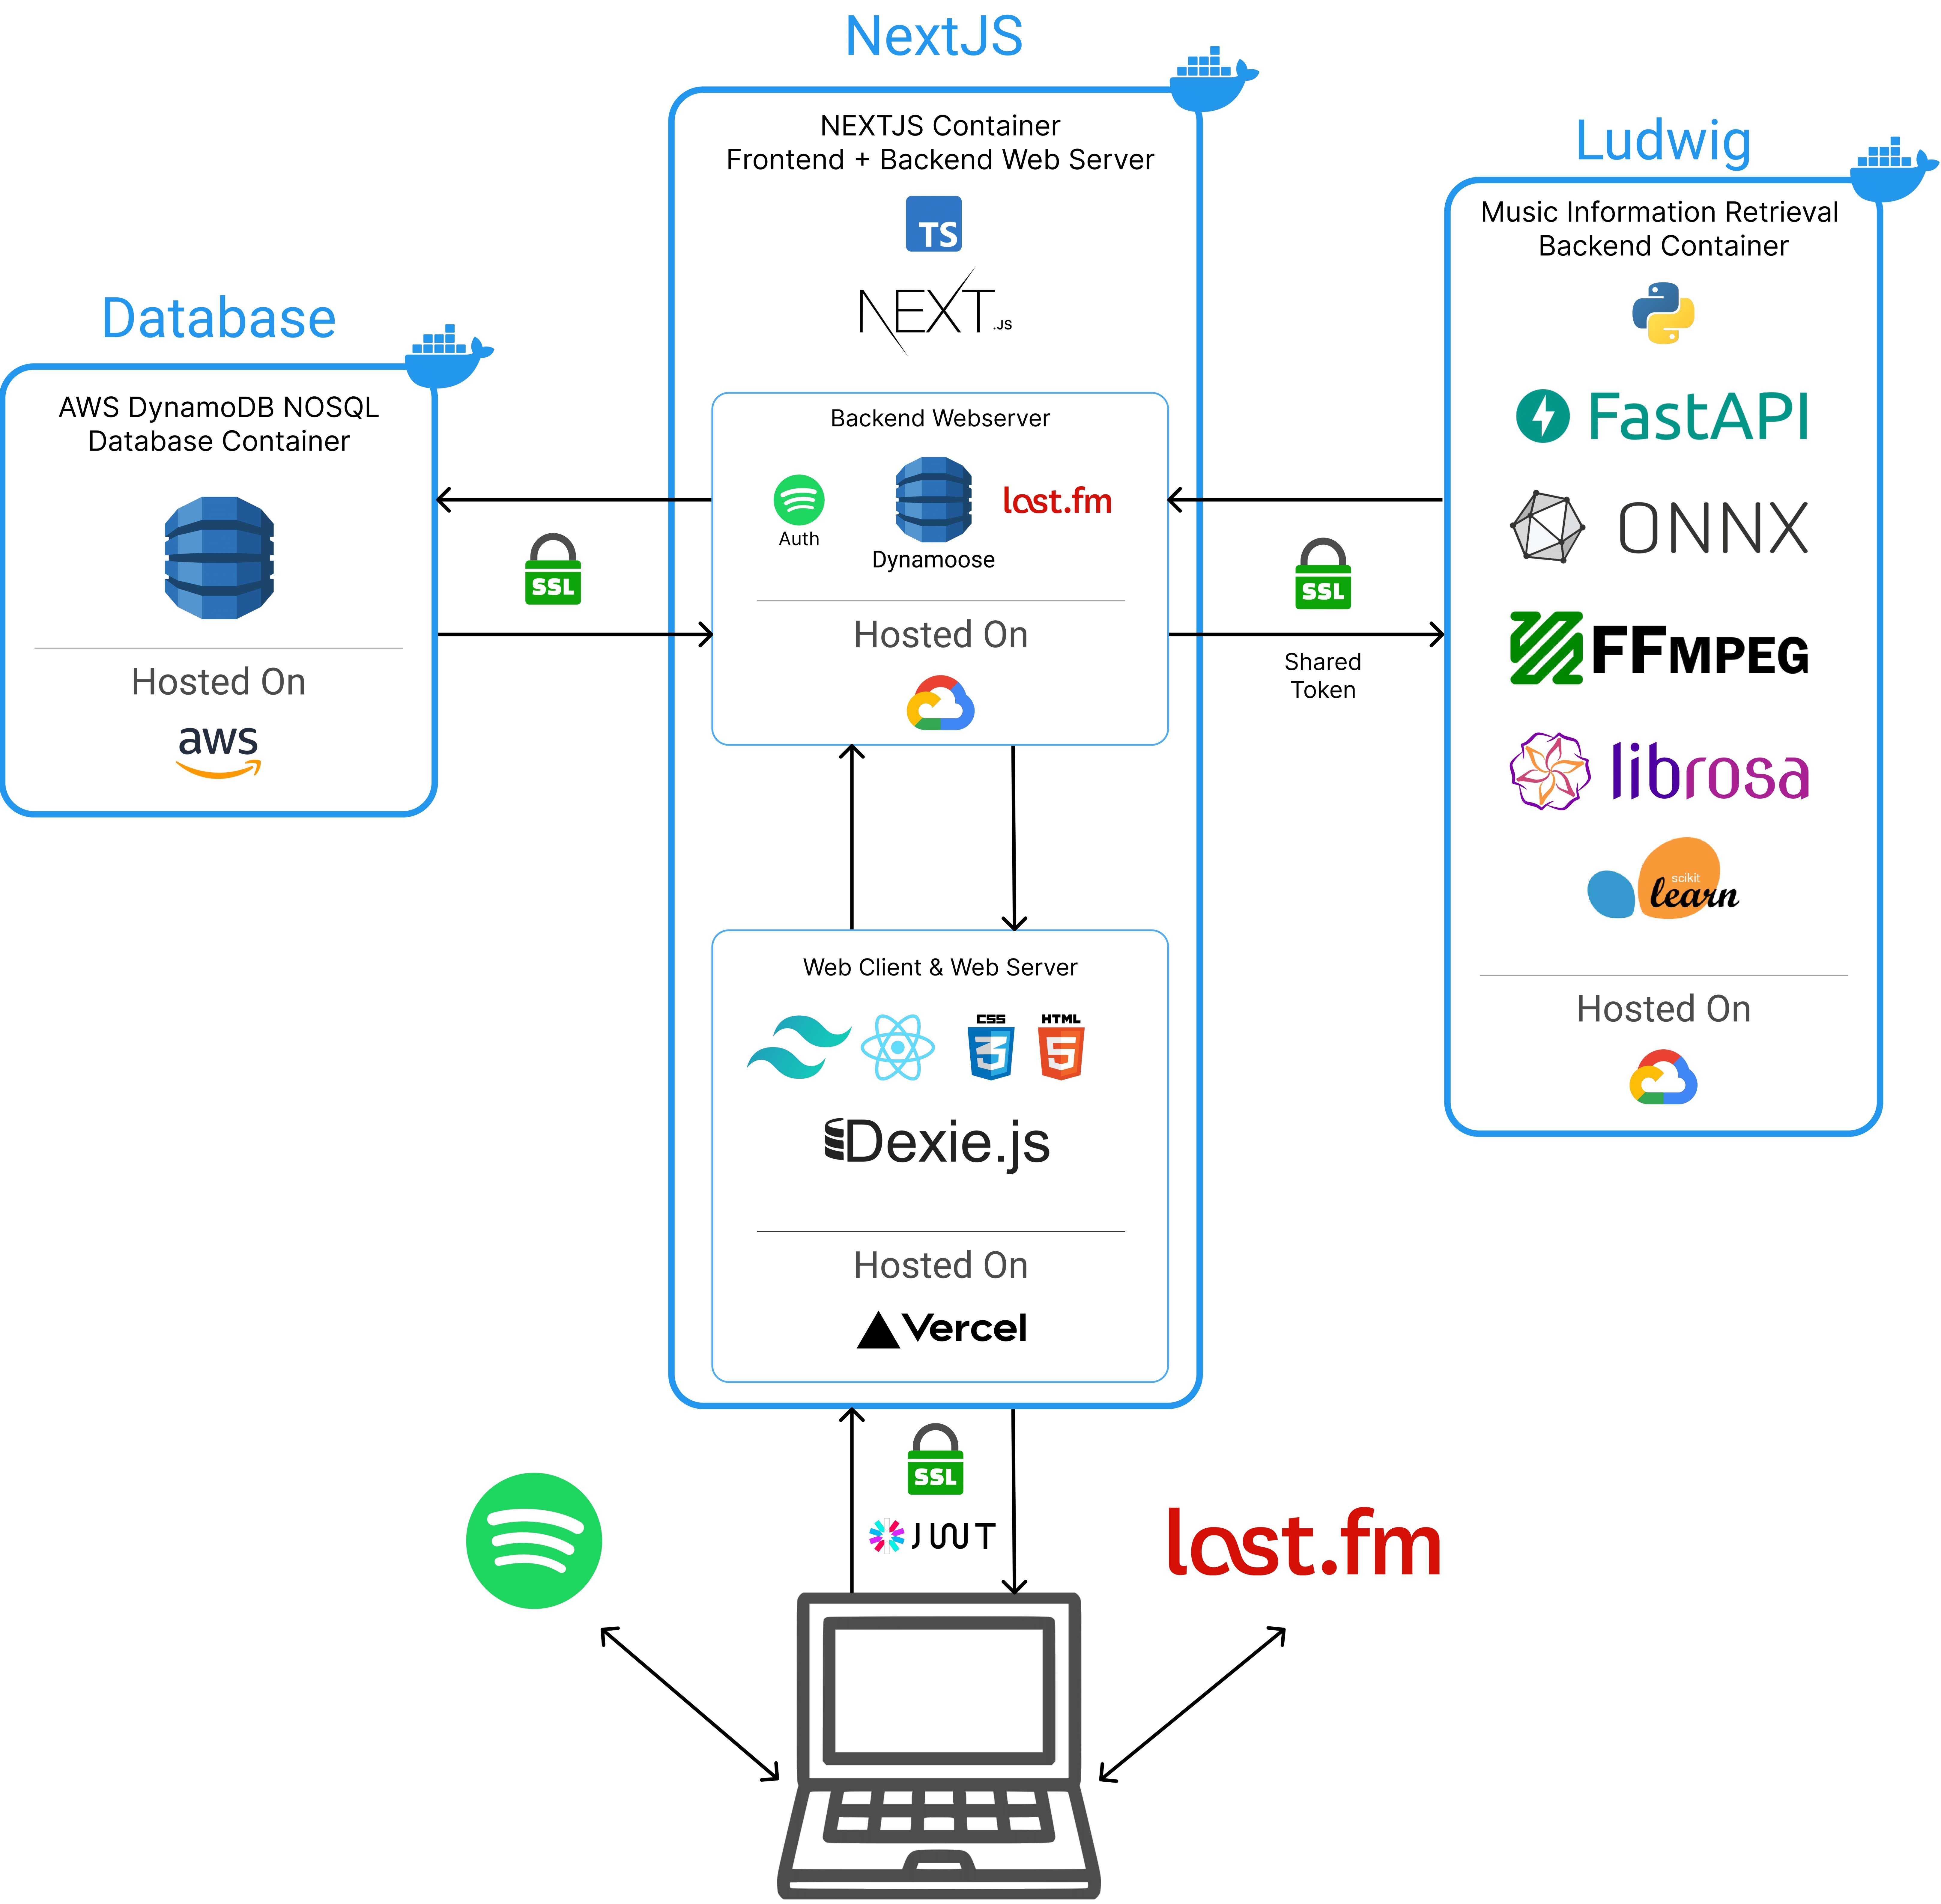
\includegraphics[width=0.9\textwidth,keepaspectratio]{img/arch_full.jpg}
    \caption{Arquitectura del Proyecto}
    \label{fig:arquitectura_contenedores}
\end{figure}

Se ha desplegado el proyecto en \href{https://spotmyfm.jorgeruizdev.com}{spotmyfm.jorgeruizdev.com} con una pequeña demo interactiva sin necesidad de registro con algunas de las funcionalidades. 

\subsection{Estructura de la Memoria}

\begin{enumerate}
    \item \textbf{Introducción}: Descripción del proyecto y estructura de la documentación.
    \item \textbf{Objetivos del Proyecto}: Objetivos generales, personales y técnicos que se esperan cumplir con este proyecto.
    \item \textbf{Conceptos Teóricos}: Explicación detallada sobre los conceptos más importantes del proyecto.
    \item \textbf{Técnicas y Herramientas}: Listado y descripción de bibliotecas, servicios y técnicas utilizados durante el proyecto, así como una breve justificación y explicación de su uso. 
    \item \textbf{Aspectos Relevantes}: Listado de los puntos más interesantes e importantes que han surgido durante el desarrollo del proyecto. 
    \item \textbf{Trabajos Relacionados}: Exposición de trabajos y plataformas relacionadas con SpotMyFM. 
    \item \textbf{Conclusiones y Lineas de Trabajo Futuras}: Conclusiones sobre los distintos aparatados del proyecto y un planteamiento de las mejoras que puede recibir el proyecto a lo largo del tiempo.
\end{enumerate}



\subsection{Estructura de los Anexos}

\begin{enumerate}[A.]
    \item \textbf{Plan del proyecto}: Plan de proyecto software que estudia la planificación y viabilidad del proyecto. 
    \item \textbf{Especificación de Requisitos}: Catálogo de los requisitos funcionales y no funcionales del proyecto.
    \item \textbf{Especificación de Diseño}: Diseño general de los distintos apartado del sistema así como su justificación.
    \item \textbf{Manual de Programador}: Manual con toda la información importante que permita a otro programado retomar el proyecto rápidamente.
    \item \textbf{Manual de Usuario}: Manual de usuario que explora todas las características de la plataforma web. 
\end{enumerate}

\subsection{Otros Materiales}

Todos los materiales están disponibles en los USBs con las fuentes. 

\begin{enumerate}
    \item \textbf{Datasets}: Contiene los distintos conjuntos de datos utilizados para los sistemas de clasificación y recomendación. 
    \item \textbf{NextJS}: Contiene la aplicación de Frontend y Backend Principal.
    \item \textbf{Ludwig}: Contiene las herramientas, notebooks y backend utilizados para el servicio de recuperación de la información musical y recomendación.
    \item \textbf{Docker}: Contiene un fichero \textbf{tcompose.yml} que permite levantar todos los servicios automáticamente.
    \item \textbf{Manual}: Contiene un fichero \textbf{readme.md} principal con el manual de la plataforma. Este fichero enlaza con archivos locales markdown más concretos que detallan una funcionalidad o vista.
    \item \textbf{Docs}: Contiene los diagramas, ficheros fuente \LaTeX de la memoria y la guía de estilo. 
\end{enumerate}